
In 1928, just two years after Erwin Schr\"odinger published his famous wave equation, Felix Bloch\footnote{At the age of 24} proposed a new method for calculating the electronic properties of solids. By this point, the idea that electrons in atoms arranged themselves into a hierarchy of discrete orbitals was well-established. Bloch proposed that, rather than starting with a free electron and considering how its motion might be affected by the potential in a material, the properties might be better understood by starting with a set of electronic states $\ket{\phi_n(\textbf{R}_i)}$, corresponding to the $n^{\textup{th}}$ orbitals on the atom at position $\textbf{R}_i$. Here, a wavefunction could be constructed by taking a linear combination of these orbitals. Next, the Hamiltonian operator, given by 
\begin{align} \label{eqn:schrodinger_H}
    H = \frac{\textbf{p}^2}{2m} + V
\end{align}
would be rewritten in terms of these states. By exploiting the translational symmetry in crystalline materials and considering only the lowest energy $s$ orbital, Bloch was able to solve the periodic Schr\"odinger equation and the technique -- known as the LCOM (linear combination of atomic orbitals), or tight-binding method -- paved the way for the development of band theory.

In practice, this was a spectacularly complex procedure to perform rigorously. To re-express the Hamiltonian in terms of orbitals, one had to evaluate an enormous number of integrals of the form $\braket{\phi_n(\textbf{R}_i)|H|\phi_m(\textbf{R}_j)}$ -- one for each pair of orbitals separated by each lattice translation. Thus, finding the exact form of the Hamiltonian was considered an impossible task. Rather, the utility of this method became apparent when one accepted this impossibility and just guessed the form of $H$. With just a few assumptions one could simplify the Hamiltonian to the point that it depended on only a small number of parameters. For example, one would expect the coupling between two orbitals to vanish unless they were sufficiently close as to overlap. Furthermore, by studying the symmetries in a crystalline material, one finds many couplings that must be equivalent. Thus, the game of constructing a tight binding model for a particular material became one of adjusting this small number of parameters until the model matched the properties found in experiment.

Although we started with the original form of Schr\"odinger's Hamiltonian (eqn.~\ref{eqn:schrodinger_H}), the tight-binding picture we have arrived at is a radically different world for an electron to live in. In Schr\"odinger's story, the electron exists as a wave in a fundamentally smooth world, where the potential defines a landscape through which the electron roams. However, in Bloch's story the collective properties of the electrons emerge from the overlap between a discrete lattice of orbitals. Here the landscape is more akin to an archipelago of islands, with electrons that can hop from island to island as in fig.~\ref{fig:hopping_electron}. Constructing a model in this formalism is a completely different procedure, since one must first determine the shape of the lattice -- the geography of the islands -- and only then can we build a Hamiltonian and write down the equations of motion.

\begin{figure}
    \centering
    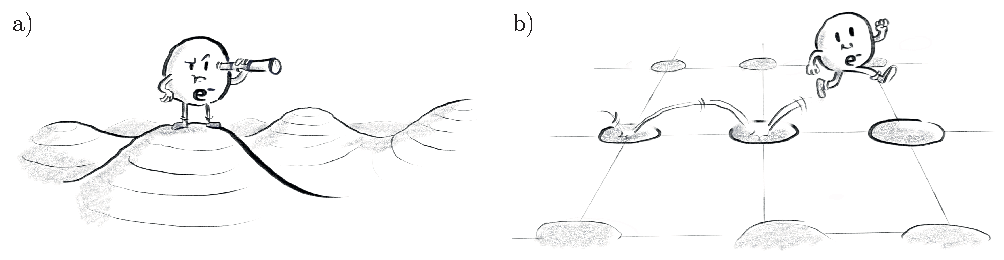
\includegraphics{introduction/figures/hopping_electron.pdf}
    \caption{
    \textbf{(a)} 
    \textbf{(b)} . 
    } 
    \label{fig:hopping_electron}
\end{figure}


% % Since the dawn of time man has gazed upon the universe and searched for answers. Some of these answers proved simple, revealing themselves after just a brief investigation. Some answers only appeared after hundreds, even thousands of years of study, passed on from generation to generation, and some answers have evaded discovery for all of time. This thesis is concerned with one of the latter questions, namely: \textit{How do the topological properties of electronic phases of matter depend on lattices upon which they are constructed?}

% % Rough opening remarks:

% When learning quantum mechanics, one's first introduction to the nature of the electron often comes in the form of the Schr\"odinger equation for a free particle:
% \begin{align}
%     i\frac{\partial}{\partial t} \ket \psi = \frac{\textbf p ^2}{2m} \ket{\psi}.
% \end{align}
% Here the electron exists as an isolated object, wandering a smooth empty expanse. Perhaps, with the addition of a potential $V$, this environment may become populated with objects, forces or even other electrons with whom to interact. Starting with this picture, one is invited to view the world inhabited by these particles as a (sometimes strong) perturbation away from a smooth and uniform place. In many branches of physics this remains a helpful story, after all -- as far as we know -- the world \textit{is} smooth and mostly empty.  

% However, for an electron that lives in a solid this picture can be deeply misleading. Here the shape of the landscape -- defined by the arrangement of atoms and the presence of other electrons -- can be the most important factor in defining the properties of the system. In many materials, the potential well at each atom is sufficiently deep that electrons remain tightly confined to them. Thus our smooth and continuous world is broken up into a set of islands, each hosting a collection of localised states that can be inhabited. Now, collective electronic properties emerge from the overlap between these localised states -- allowing the electrons to hop from site to site, or realign their spin and internal degrees of freedom in response to the state of a neighbour. In the most extreme example, the electron-electron repulsion can be strong enough that electrons are completely forbidden from hopping from one atom to a neighbour -- forming a so-called Mott insulator \cite{mott_basis_1949}. 


% Thus, rather than treating the environment as a potential in a smooth world, it is more useful to view the electrons as moving between a set of isolated islands arranged on the vertices of a discretised lattice defined by the background material. This intuition forms the 

% % tight-binding model, where the equations of motion are built on the assumption that electrons exist only on a discretised lattice defined by the background material. 
% % Finally, in certain materials, the electron-electron interaction is such that electrons are immobilised at each site -- mott insulators -- and the system has truly separated into a lattice of individual sites hosting individual electrons, interacting with one another primarily through the overlap of their wavefunctions. 
% % In the weak limit this background can be seen as a gentle perturbation on the motion of an otherwise free particle, however in many materials the opposite is true -- the electronic properties of the material are formed by the overlap of outer orbitals in the atoms, and the lattice can be seen rather as fundamental in defining the ways electrons can exist inside a material. Here the electrons are strongly localised to individual atoms, or can jump from atom to atom, and is described by a tight binding model -- viewing each atom as a site that can hold number of electrons in well-defined states. 

% In these materials, where electrons are constrained in their movement by the structure of their hosting material, an understanding of their collective properties requires two ingredients: The microscopic interactions that describe how electrons interact with their surroundings and each other, and the geometry of the lattice on which they live. Thus, a natural question to ask is `How does the shape of these lattices affect the ways that electrons can order within them'. It is this question that motivates 

% Historically, this question this has proved to be an extremely rich question, with an astonishing variety of answers depending on the material and the microscopic interaction terms. 

% There are examples of materials where the properties of the electron phases are remarkably insensitive to lattice geometry, and the same type of Hamiltonian defined on any lattice will produce largely the same physics. A rather obvious example are ferromagnetic materials, where the spins forming the material will align regardless of the microscopics of the lattice. Even on different lattices, the Ising model has been shown to have identical behaviour in the thermodynamic limit, where the universality class remains unaffected by local changes in lattice. More recently, a new class of remarkably insensitive phenomena emerged -- the quantum Hall effect. Here, the bulk conductance of the electrons is quantised to a precise value, regardless of the presence of disorder in the system. Here, the Hamiltonian defined on any lattice will have largely the same properties and the presence of disorder serves not to disrupt but to stabilise the universal nature of these materials properties. 

% At the other extreme are materials where the same Hamiltonian defined on different lattices can give wildly different results. An example is the antiferromagnetic Heisenberg model, which can give N\'eel, VBS and was even proposed as a possible spin liquid phase on a sufficiently geometrically frustrated lattice. 
